\documentclass[12pt]{article}
\usepackage[none]{hyphenat}
\usepackage{fontspec}
\usepackage{geometry}
\usepackage{enumitem}
\usepackage{titlesec}
\usepackage{tikz}
\usepackage{amsmath}
\usepackage{array}
\usepackage{longtable}
\usepackage{xcolor}
\usepackage{listings}
\usepackage{float}
\usetikzlibrary{calc, shapes.geometric, arrows, positioning}

\setmainfont{TH Sarabun New}
\geometry{a4paper, margin=1in}

\tikzset{
    entity/.style={rectangle, draw, minimum width=2.5cm, minimum height=1cm, text centered, thick},
    weakEntity/.style={rectangle, draw, double, minimum width=2.5cm, minimum height=1cm, text centered, thick},
    relationship/.style={diamond, draw, aspect=2, minimum width=2.5cm, text centered, thick},
    identRelationship/.style={diamond, draw, double, aspect=2, minimum width=2.5cm, text centered, thick},
    attribute/.style={ellipse, draw, minimum width=1.5cm, text centered, thin},
    keyAttribute/.style={ellipse, draw, thick, text centered},
    partialKey/.style={ellipse, draw, dashed, text centered, thin},
    isa/.style={isosceles triangle, draw, shape border rotate=90, minimum width=1.5cm, minimum height=1cm, text centered, thick}
}

\lstset{
    basicstyle=\ttfamily\small,
    breaklines=true,
    frame=single,
    rulecolor=\color{black!30},
    backgroundcolor=\color{gray!5},
    language=SQL,
    keywordstyle=\color{blue}
}

\begin{document}
\sloppy

\begin{center}
    \rule{\textwidth}{1pt} \\
    \textbf{\Large Mock Exam: CPE241 Database Systems (Module 1)} \\
    \textbf{Lectures 1-5: Advanced Theory \& Modeling Analysis} \\
    \textbf{\textcolor{red}{ULTRA HARD MODE - Senior Layout Format}} \\
    \rule{\textwidth}{1pt}
\end{center}

\section*{Part 1: Multiple Choice (English) - 20 Marks}
\begin{enumerate}
    \item In the context of Concurrency Control, a "Wait-for Graph" is primarily used to detect:
    \begin{enumerate}[label=\alph*)]
        \item Cascading rollbacks \quad \item Deadlock \quad \item Phantom reads \quad \item Dirty writes
    \end{enumerate}

    \item If you change the underlying data structures (e.g., using B-trees instead of Hashing) without affecting the Conceptual Schema, you are demonstrating:
    \begin{enumerate}[label=\alph*)]
        \item Physical Data Independence \quad \item Logical Data Independence \quad \item Internal Consistency \quad \item View Authorization
    \end{enumerate}

    \item An "Alternate Key" is defined as:
    \begin{enumerate}[label=\alph*)]
        \item A Foreign Key that points to a non-primary key \quad \item A Candidate Key not chosen as the Primary Key \quad \item A key that is used only for sorting \quad \item A composite key with redundant attributes
    \end{enumerate}

    \item What is the critical difference between a Weak Entity and a Strong Entity?
    \begin{enumerate}[label=\alph*)]
        \item Weak entities cannot have relationships \quad \item Weak entities lack sufficient attributes to form a primary key of their own \quad \item Weak entities must have double-circle attributes \quad \item Weak entities are only used in 1:1 relationships
    \end{enumerate}

    \item The SQL \texttt{DROP TABLE} statement belongs to which sub-language category?
    \begin{enumerate}[label=\alph*)]
        \item Data Manipulation Language (DML) \quad \item Data Definition Language (DDL) \quad \item Data Control Language (DCL) \quad \item Transaction Control Language (TCL)
    \end{enumerate}

    \item How is a "Multi-valued Attribute" typically handled when mapping to a Relational Schema?
    \begin{enumerate}[label=\alph*)]
        \item By adding multiple columns to the existing table \quad \item By creating a new table and linking it via a Foreign Key \quad \item By merging it into the Primary Key \quad \item By ignoring the attribute
    \end{enumerate}

    \item In ER modeling, a relationship with a degree of three represents:
    \begin{enumerate}[label=\alph*)]
        \item A recursive relationship \quad \item A triple-binary relationship \quad \item A ternary relationship \quad \item A high-level generalization
    \end{enumerate}

    \item Which notation represents "Total Participation" in a standard Chen ER Diagram?
    \begin{enumerate}[label=\alph*)]
        \item Single line \quad \item Dotted line \quad \item Double line \quad \item Bold arrow
    \end{enumerate}

    \item The DBMS component that stores metadata and constraints is known as the:
    \begin{enumerate}[label=\alph*)]
        \item Query Optimizer \quad \item System Catalog / Data Dictionary \quad \item Transaction Log \quad \item Storage Engine
    \end{enumerate}

    \item To store a Many-to-Many (M:N) relationship between two entities, how many tables are required at minimum?
    \begin{enumerate}[label=\alph*)]
        \item 1 \quad \item 2 \quad \item 3 \quad \item 4
    \end{enumerate}

    \item Which component of a DBMS is primarily responsible for ensuring Atomicity and Durability?
    \begin{enumerate}[label=\alph*)]
        \item Query Processor \quad \item Buffer Manager \quad \item Transaction Manager \quad \item Network Manager
    \end{enumerate}

    \item The Referential Integrity rule states that:
    \begin{enumerate}[label=\alph*)]
        \item A Primary Key must be unique \quad \item A Foreign Key must match a Primary Key in the referenced table, or be NULL \quad \item Every table must have a Primary Key \quad \item Data types must be consistent across the database
    \end{enumerate}

    \item In the 3-Schema Architecture, physical file organization and indexing are defined in the:
    \begin{enumerate}[label=\alph*)]
        \item External Schema \quad \item Conceptual Schema \quad \item Internal Schema \quad \item User Schema
    \end{enumerate}

    \item A "Composite Attribute" is defined as an attribute that:
    \begin{enumerate}[label=\alph*)]
        \item Can have multiple values for a single entity \quad \item Can be further subdivided into smaller component attributes \quad \item Is derived from other stored attributes \quad \item Is a combination of two primary keys
    \end{enumerate}

    \item The process of converting requests between different levels of the database architecture is called:
    \begin{enumerate}[label=\alph*)]
        \item Optimization \quad \item Mapping \quad \item Normalization \quad \item Encapsulation
    \end{enumerate}

    \item In an EER Diagram, a circle with an "o" symbol represents which constraint?
    \begin{enumerate}[label=\alph*)]
        \item Disjoint constraint \quad \item Overlapping constraint \quad \item Total participation \quad \item Partial participation
    \end{enumerate}

    \item How does a "Derived Attribute" differ from a "Stored Attribute"?
    \begin{enumerate}[label=\alph*)]
        \item It is not physically stored in the database \quad \item It is always a primary key \quad \item It cannot be updated \quad \item It is only used in weak entities
    \end{enumerate}

    \item "Data Isolation" in traditional file systems refers to the problem where:
    \begin{enumerate}[label=\alph*)]
        \item Data is too secure \quad \item Data is spread across different files and formats, making it difficult to link \quad \item Data is duplicated excessively \quad \item Data is lost during transmission
    \end{enumerate}

    \item In Crow's Foot notation, a small circle on the relationship line represents:
    \begin{enumerate}[label=\alph*)]
        \item Mandatory (1) \quad \item Optional (0) \quad \item Many \quad \item Primary Key
    \end{enumerate}

    \item When a crash occurs, which log is used by the DBMS to perform a recovery?
    \begin{enumerate}[label=\alph*)]
        \item Error Log \quad \item Audit Log \quad \item Transaction Log (Undo/Redo Log) \quad \item Metadata Log
    \end{enumerate}
\end{enumerate}

\newpage
\section*{Part 2: Analytical Short Answer (ภาษาไทย) - 20 Marks}
\begin{enumerate}[itemsep=1cm]
    \item จงอธิบายปรากฏการณ์ "Lossless Join" และความสำคัญในการรักษาความถูกต้องของข้อมูล
    \item "Deadlock" เกิดขึ้นได้อย่างไรในระบบฐานข้อมูล และ DBMS มีวิธีจัดการเบื้องต้นอย่างไร?
    \item "Natural Join" ต่างจาก "Inner Join" ทั่วไปอย่างไรในเชิงโครงสร้าง (Lect. 4)?
    \item ในการออกแบบ ERD, การเลือกระหว่าง "Attribute" และ "Entity" มีเกณฑ์การตัดสินใจอย่างไร?
    \item จงระบุความแตกต่างระหว่าง "Generalization" และ "Specialization" ใน EER Modeling
    \item เพราะเหตุใดจึงควรใช้ BCNF แทนที่ 3NF ในบางกรณี (อธิบายหลักการเบื้องต้น)?
    \item จงอธิบาย "Data Abstraction" 3 ระดับ และความสัมพันธ์กับ Data Independence
    \item "Weak Entity" สามารถมี Weak Entity ของตัวเองซ้อนลงไปอีกชั้นได้หรือไม่? จงยกตัวอย่างประกอบ
    \item จงบอกความหมายของ "Surrogate Key" และสถานการณ์ที่ควรหลีกเลี่ยงการใช้งาน
    \item ใน EER, "Disjoint Constraint (d)" ช่วยลดปัญหา Inconsistency ได้อย่างไร?
\end{enumerate}

\newpage
\section*{Part 3: Practical Design Challenge (ภาษาไทย) - 20 Marks}

\begin{enumerate}[label=\textbf{ข้อที่ \arabic*.}]
    \item \textbf{High-Level SQL \& Schema Implementation (10 Marks):} 
    จงเขียนชุดคำสั่ง SQL เพื่อสร้างโครงสร้างพื้นฐานสำหรับระบบ "Order Management" โดยสังเกตจากสถานะข้อมูลในตารางต่อไปนี้:

    \begin{minipage}{0.48\textwidth}
    \textbf{Table: \texttt{CUSTOMERS}} \\
    {\small
    \begin{tabular}{|l|l|l|}
    \hline \textbf{cid (PK)} & \textbf{name} & \textbf{email (Unique)} \\
    \hline C01 & Somsak & s@kmutt.ac.th \\
    \hline C02 & Somying & y@kmutt.ac.th \\
    \hline
    \end{tabular}
    }
    \end{minipage}
    \begin{minipage}{0.48\textwidth}
    \textbf{Table: \texttt{ORDERS}} \\
    {\small
    \begin{tabular}{|l|l|l|}
    \hline \textbf{oid (PK)} & \textbf{cid (FK)} & \textbf{total\_amt} \\
    \hline OR-99 & C01 & 1,500.00 \\
    \hline OR-88 & C02 & 2,200.00 \\
    \hline
    \end{tabular}
    }
    \end{minipage}

    \vspace{0.4cm}
    \textbf{Table: \texttt{LINE\_ITEMS} (Composite Primary Key)}
    {\small
    \begin{center}
    \begin{tabular}{|l|l|l|l|}
    \hline \textbf{oid (FK)} & \textbf{item\_id} & \textbf{prod\_name} & \textbf{qty (CHECK > 0)} \\
    \hline OR-99 & 1 & Laptop & 1 \\
    \hline OR-99 & 2 & Mouse & 2 \\
    \hline OR-88 & 1 & Keyboard & 1 \\
    \hline
    \end{tabular}
    \end{center}
    }

    \textbf{โจทย์:} จงเขียน SQL DDL และ DML เพื่อดำเนินการดังนี้:
    \begin{enumerate}[label=\roman*)]
        \item สร้างตารางทั้ง 3 โดยมีเงื่อนไข: \texttt{total\_amt} ห้ามน้อยกว่า 0, \texttt{email} ห้ามซ้ำ, และถ้าลบ Order ข้อมูลใน Line Items ต้องหายไปด้วย (\textbf{ON DELETE CASCADE})
        \item เพิ่มคอลัมน์ \texttt{status} (Default = 'Pending') ในตาราง ORDERS โดยใช้คำสั่ง \texttt{ALTER}
        \item เขียนคำสั่ง INSERT ข้อมูลลงในตาราง \texttt{LINE\_ITEMS} สำหรับแถวที่มี \texttt{oid} 'OR-99' และ \texttt{item\_id} 1
    \end{enumerate}
    
    \textbf{พื้นที่เขียนคำตอบ:}
    \begin{lstlisting}[frame=single, minheight=6cm]
-- 1. Create Tables

-- 2. Alter Table

-- 3. Insert Data

    \end{lstlisting}

    \newpage
    \item \textbf{Advanced EER Modeling (10 Marks):}
    จงวาด Conceptual Diagram สำหรับระบบ "Fleet Management":
    \begin{itemize}
        \item \texttt{Vehicle} มี \underline{ChassisID}, \texttt{Brand}
        \item แบ่งเป็น \texttt{Car} (Doors) และ \texttt{Truck} (Capacity) แบบ \textbf{Disjoint \& Total (Mandatory)}
        \item ยานพาหนะต้องมี \texttt{Owner} (รหัส, ชื่อ) 1 คน รถ 1 คันมีเจ้าของได้หลายคน (M:N) โดยต้องเก็บวันที่เริ่มครอบครอง (\texttt{StartDate})
        \item \texttt{Maintenance} เป็น \textbf{Weak Entity} ขึ้นกับ \texttt{Vehicle} (เลขที่ซ่อม, ค่าใช้จ่าย)
    \end{itemize}
    
    \vspace{0.5cm}
    \centerline{\fbox{\begin{minipage}[c][12cm]{15cm} \centering (วาด EER Diagram ตรงนี้ - เน้นความถูกต้องของ Hierarchy และ Weak Entity) \end{minipage}}}
\end{enumerate}

\newpage
\begin{center}
    \rule{\textwidth}{2pt} \\
    \textbf{\Large เฉลยละเอียด (ULTRA HARD MODE Senior Solution)} \\
    \rule{\textwidth}{2pt}
\end{center}

\subsection*{Part 1: MCQ Explanations}
\begin{longtable}{|c|c|p{10cm}|}
\hline \textbf{No.} & \textbf{Ans} & \textbf{Explanation} \\ \hline
1 & b & Wait-for Graph เป็นกราฟที่แสดงการรอทรัพยากรระหว่าง Transaction ถ้าเป็นวงกลม (Cycle) แสดงว่าเกิด Deadlock \\ \hline
2 & a & Physical Data Independence คือการเปลี่ยนโครงสร้างระดับ Internal (เช่น Index, File structure) โดยไม่กระทบ Conceptual \\ \hline
3 & b & Alternate Key คือ Candidate Key ที่มีคุณสมบัติระบุตัวตนได้ครบถ้วนแต่ไม่ได้ถูกเลือกเป็น Primary Key \\ \hline
4 & b & Weak Entity ขาด identity ของตัวเอง จำเป็นต้องอาศัย Owner Entity และ Partial Key เพื่อสร้างคีย์หลักชุดสมบูรณ์ \\ \hline
5 & b & DDL (Data Definition Language) จัดการโครงสร้าง Schema; DROP คือการถอนโครงสร้างทั้งหมดออกจากระบบ \\ \hline
6 & b & 1NF กำหนดให้ข้อมูลในคอลัมน์ต้องเป็น Atomic การมี Multi-valued ต้องแยกตารางเพื่อลด Redundancy \\ \hline
7 & c & Degree = จำนวน Entity Types ที่เข้าร่วมใน Relationship; 3 = Ternary \\ \hline
8 & c & เส้นคู่ (Double Line) แทนการมีส่วนร่วมแบบเบ็ดเสร็จ (Total Participation) หรือ Mandatory \\ \hline
9 & b & System Catalog/Data Dictionary เก็บ Metadata ทั้งหมดของฐานข้อมูล \\ \hline
10 & c & ตาราง A + ตาราง B + ตาราง Junction (Link Table) สำหรับ Many-to-Many = 3 ตาราง \\ \hline
11 & c & Transaction Manager ดูแลเรื่องความถูกต้องของธุรกรรมตามกฎ ACID (Atomicity, Isolation, Durability) \\ \hline
12 & b & Referential Integrity บังคับความสัมพันธ์ระหว่างคีย์ FK ต้องอ้างไปเจอ PK ที่มีอยู่จริงเพื่อความปลอดภัย \\ \hline
13 & c & Internal Schema จัดการเรื่องการเก็บข้อมูลทางกายภาพ เช่น การระบุที่อยู่ของ Record บน Disk \\ \hline
14 & b & Composite attribute คือคุณลักษณะที่ยังสามารถแบ่งย่อยลงไปได้อีก เช่น ชื่อ (ประกอบด้วยชื่อจริงและนามสกุล) \\ \hline
15 & b & Mapping คือการระบุความเชื่อมโยงระหว่างชั้นต่างๆ ของ 3-Schema Architecture \\ \hline
16 & b & Overlap (o) หมายถึงข้อมูลหนึ่งตัวสามารถเป็นสมาชิกของหลาย Subclass ได้ในเวลาเดียวกัน \\ \hline
17 & a & Derived Attribute คือค่าที่ได้จากการนำข้อมูลอื่นมาประมวลผล (Runtime calculation) จึงไม่เก็บลงดิสก์จริง \\ \hline
18 & b & Data Isolation ในระบบเก่าคือข้อมูลที่กระจัดกระจายอยู่ในหลายไฟล์และหลายฟอร์แมต ทำให้เชื่อมโยงยาก \\ \hline
19 & b & วงกลม (Circle) ใน Crow's Foot หมายถึงค่า 0 หรือ Optional \\ \hline
20 & c & Transaction Log บันทึกทุกการเปลี่ยนแปลงเพื่อใช้ในการ Undo/Redo เมื่อระบบล่มหรือต้องการ Rollback \\ \hline
\end{longtable}

\subsection*{Part 2: Analytical Short Answer Key}
\begin{enumerate}
    \item \textbf{Lossless Join:} คือเงื่อนไขที่เมื่อเรา Decompose ตารางหนึ่งออกเป็นสองตารางแล้ว เมื่อนำมา Join กันกลับด้วยเงื่อนไขที่ถูกต้อง ผลลัพธ์ต้องได้เหมือนเดิมเป๊ะ หากเกิดข้อมูลเกิน (Spurious Tuples) จะเป็น Lossy ซึ่งทำลายความถูกต้องของข้อมูล
    \item \textbf{Deadlock:} เกิดเมื่อ T1 รอ B (ที่ T2 ถือ) และ T2 รอ A (ที่ T1 ถือ) วนเป็นวงกลม วิธีแก้คือ Deadlock Detection (Wait-for graph) แล้วทำ Rollback ตัวที่มีค่าความเสียหายน้อยที่สุด (Victim selection)
    \item \textbf{Natural Join vs Inner Join:} Natural Join จะทำการเปรียบเทียบคอลัมน์ที่ชื่อเหมือนกันโดยอัตโนมัติ และกำจัดคอลัมน์ที่ซ้ำซ้อนให้เหลือเพียงอันเดียว ต่างจาก Inner Join ที่มักจะคงไว้ทั้งสองฝั่งหากไม่ได้ระบุ SELECT
    \item \textbf{Attribute vs Entity:} พิจารณาจาก "รายละเอียด" หากต้องการเก็บข้อมูลย่อยๆ ของสิ่งนั้น (Attributes) และมันมีความสัมพันธ์กับคนอื่น สิ่งนั้นควรเป็น Entity แต่หากเป็นเพียงค่าค่าเดียว สิ่งนั้นเป็น Attribute
    \item \textbf{Gen vs Spec:} \textbf{Specialization} (บนลงล่าง) แยกกลุ่มใหญ่ออกเป็นกลุ่มย่อยที่เจาะจง \textbf{Generalization} (ล่างขึ้นบน) รวมกลุ่มย่อยที่มีจุดร่วมกันขึ้นเป็นกลุ่มฐานข้อมูลเดียวกัน
    \item \textbf{BCNF vs 3NF:} 3NF ยอมให้ Determinant ไม่เป็น Superkey ได้หากเป็นส่วนของคีย์ CK แต่ BCNF บังคับว่า "ทุก Determinant ต้องเป็น Superkey" เท่านั้นเพื่อกำจัดความซ้ำซ้อนระดับสูง
    \item \textbf{Data Abstraction:} External (หน้าจอยูสเซอร์), Conceptual (โครงสร้างเนื้อหา), Internal (การเก็บจริง) การแยกชั้นช่วยให้แก้ไขส่วนล่างได้โดยไม่กระทบส่วนบน (Data Independence)
    \item \textbf{Multi-level Weak Entity:} \textbf{ได้} เช่น Building (Strong) -> Room (Weak) -> Computer (Weak ขึ้นกับ Room) โดย Computer ต้องมี PK ที่รวมมาจากทั้ง Building และ Room
    \item \textbf{Surrogate Key:} คีย์ที่ระบบสร้างให้เอง (Auto-increment) ข้อดีคือเร็วและแน่นอน แต่ควรเลี่ยงหากข้อมูลมี Natural Key ที่มั่นคงและสื่อความหมายชัดเจนอยู่แล้ว เพื่อลดภาระการ JOIN ตาราง
    \item \textbf{Disjoint (d):} บังคับว่า Instance หนึ่งย้ายไปอยู่ได้เพียง Subclass เดียวเท่านั้น ป้องกันการทำข้อมูลซ้ำซ้อนและช่วยให้การ Check Inconsistency ทำได้ง่ายขึ้น
\end{enumerate}

\newpage
\subsection*{Part 3: Practical Solution Details}

\textbf{1. Advanced SQL Solution:}
\begin{lstlisting}[language=SQL]
-- i) Create Tables with Constraints
CREATE TABLE CUSTOMERS (
    cid CHAR(3) PRIMARY KEY,
    name VARCHAR(50) NOT NULL,
    email VARCHAR(100) UNIQUE
);

CREATE TABLE ORDERS (
    oid CHAR(5) PRIMARY KEY,
    cid CHAR(3) REFERENCES CUSTOMERS(cid),
    total_amt DECIMAL(10,2) CHECK (total_amt >= 0)
);

CREATE TABLE LINE_ITEMS (
    oid CHAR(5) REFERENCES ORDERS(oid) ON DELETE CASCADE,
    item_id INT,
    prod_name VARCHAR(50),
    qty INT CHECK (qty > 0),
    PRIMARY KEY (oid, item_id)
);

-- ii) Alter Table
ALTER TABLE ORDERS ADD status VARCHAR(20) DEFAULT 'Pending';

-- iii) Insert Data
INSERT INTO LINE_ITEMS (oid, item_id, prod_name, qty) 
VALUES ('OR-99', 1, 'Laptop', 1);
\end{lstlisting}

\vspace{0.5cm}
\textbf{2. EER Diagram Solution (TikZ Logic):}
\begin{center}
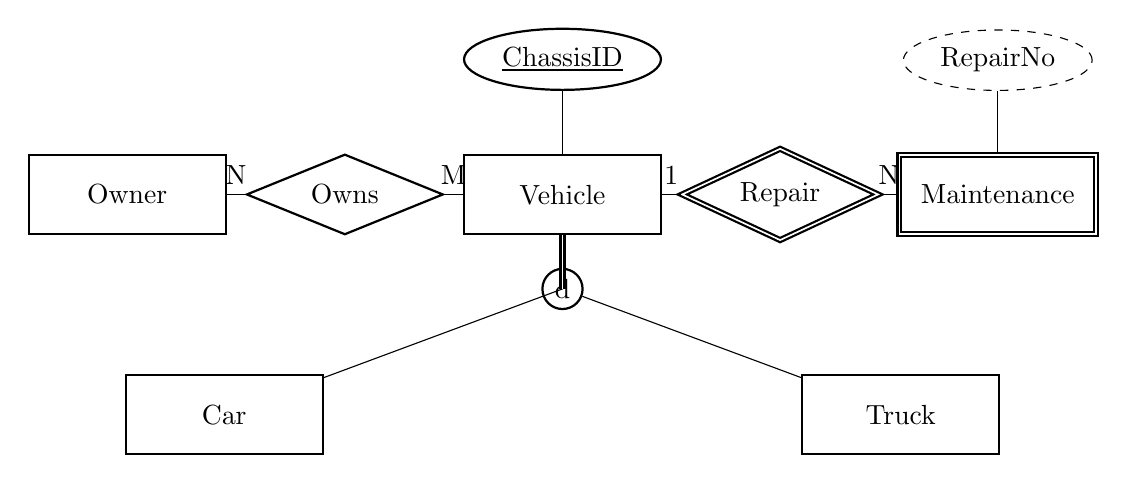
\begin{tikzpicture}[node distance=2.5cm, every edge/.style={draw, thick}]
    \node[entity] (vh) {Vehicle};
    \node[entity] (car) [below left=of vh] {Car};
    \node[entity] (truck) [below right=of vh] {Truck};
    \node[entity] (owner) [left=3cm of vh] {Owner};
    \node[weakEntity] (maint) [right=3cm of vh] {Maintenance};
    
    % Hierarchy
    \draw (vh) -- ++(0,-1.2) node[circle, draw, thick, inner sep=2pt] (d) {d} -- (car);
    \draw (d) -- (truck);
    \draw[double, thick] (vh.south) -- (0, -1.2); 
    
    \node[relationship] (owns) at ($(owner)!0.5!(vh)$) {Owns};
    \node[identRelationship] (has) at ($(vh)!0.5!(maint)$) {Repair};
    
    \draw (owner) -- (owns) node[midway, above] {N};
    \draw (owns) -- (vh) node[midway, above] {M};
    \draw (vh) -- (has) node[midway, above] {1};
    \draw (has) -- (maint) node[midway, above] {N};
    
    \node[keyAttribute] (cid) [above=0.8cm of vh] {\underline{ChassisID}};
    \node[partialKey] (mid) [above=0.8cm of maint] {\dashuline{RepairNo}};
    \draw (vh) -- (cid); \draw (maint) -- (mid);
\end{tikzpicture}
\end{center}

\end{document}
